\chapter{Analysis}\label{sec:analysis}
Sections~\ref{sec:analysis:examples:single} and~\ref{sec:analysis:examples:multiple} abstract and deduce the essential characteristics of any interaction.
These characteristics are relevant for a formalized language of \cmvs{}.
To accomplish this goal, the approach is to deduce the characteristics by a list of examples.
What are the expected data structures for each visualization?
Which visual variables can be used to show the effect of an interaction?
A list of possible interactions is given for each visualization.
Those interactions will be classified according to \textcite{Yi2007} and the relevant subject of the interaction is specified.

Section~\ref{sec:analysis:requirements} gives a set of requirements which can be used to evaluate a framework of \cmvs{}.

Finally in Section~\ref{sec:analysis:frontend-framework-comparison} the advantages and disadvantages of several web frontend frameworks are contrasted.
A final decision is made which framework will be used for the implementation of the conceptual framework.

\section{Single Visualization Interactions}\label{sec:analysis:examples:single}

The data visualization catalogue by Severino Ribecca list many of the most used data visualizations\cite{VisualizationCatalogue2017}.
This section covers a list of common data visualizations from that catalogue as examples.
The expected data structure and a list of possible interactions are systematically analysed.

\subsection{Line graphs}
\begin{figure}
  \begin{center}
    \subfloat[Line graphs]{{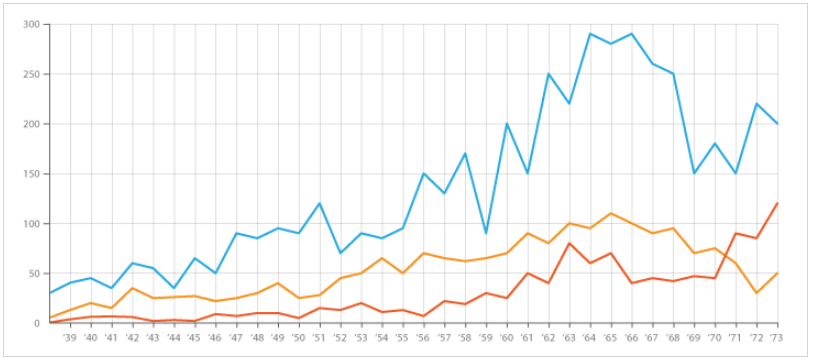
\includegraphics[width=0.4\textwidth]{figures/analysis/line-graphs} }}%
    \qquad
  \end{center}
  \caption{Line graphs are used to display trends}
  \label{fig:analysis:line-graphs}
\end{figure}

Line graphs display how quantitative values have changed over time.
They are perfectly suited to show trends or compare multiple series of data with each other.
Line graphs visualize one or many series of data in parallel and therefore the expected data format is \emph{tabular}.

Line graphs are drawn in a Cartesian coordinate system, connecting subsequent points to each other.
Thus,
\begin{enumerate*}[label=(\arabic*)]
    \item position
    \item orientation and
    \item texture
\end{enumerate*}
are constrained by the nature of the visualization.
However, an interaction with the line graph can alter the
\begin{enumerate*}[label=(\arabic*)]
    \item shape
    \item color or
    \item size
\end{enumerate*}
of lines to communicate an interaction.
It is further possible to highlight either the entire series of data or a single data point within that series, e.g. changing the shape and size of the point.
Table~\ref{tab:analysis:line-graph:interactions} shows a list of plausible interactions in a line graph.

\begin{table}[H]
  \centering
  \begin{tabular*}{\textwidth}{lll}
    \bf Category & \bf Description & \bf Exchanged information \\
    \hline
    Select & Highlight a data point & id of data point \\
    Select & Highlight a data series & id of data series \\
    Encode & Change colours of data series & id of data series + colour \\
    Filter & Restrict interval on x-axis & lower limit + upper limit \\
    Filter & Hide a data series & id of data series \\
  \end{tabular*}
  \caption{Plausible interactions for line charts}%
  \label{tab:analysis:line-graph:interactions}
\end{table}




\subsection{Bar charts and multi set bar charts}

\begin{figure}
  \begin{center}
    \subfloat[Bar chart or column graph]{{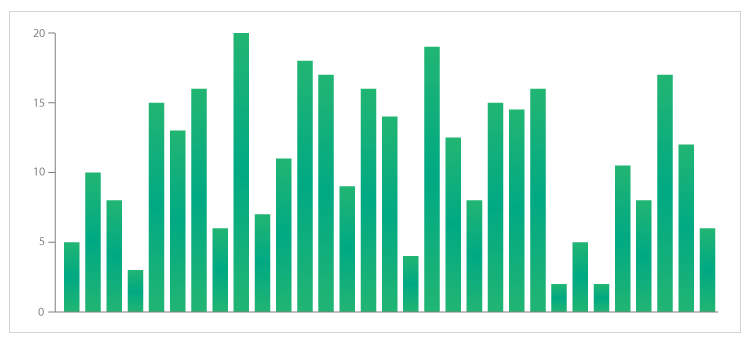
\includegraphics[width=0.4\textwidth]{figures/analysis/bar-chart} }}%
    \qquad
    \subfloat[Multi set bar chart]{{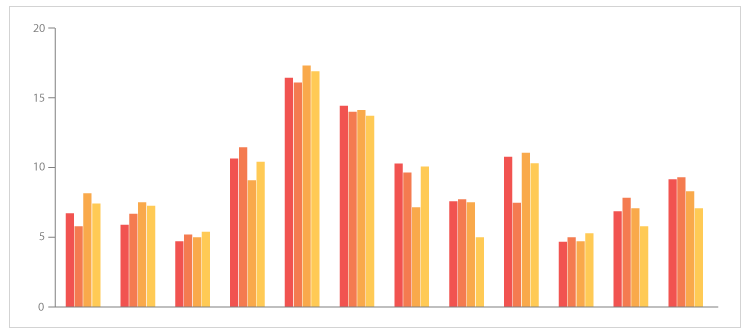
\includegraphics[width=0.4\textwidth]{figures/analysis/multiset-bar-chart} }}%
  \end{center}
  \caption{A multi set bar charts is a variation of a bar chart}
  \label{fig:analysis:bar-charts}
\end{figure}

Bar charts use either horizontal or vertical bars to show discrete, numerical comparisons across categories.
The length of a bar displays a quantitative value of a category.

Multiple bar charts display many data series next to each other.
Every series is grouped by category and a colour can be used to identify a data series.

Like line graphs, bar charts expect a \emph{tabular} data format.
In contrast to line graphs, bar charts are used to show a comparison rather than a trend.

The type of the visualization constrains the
\begin{enumerate*}[label=(\arabic*)]
    \item shape,
    \item size and, in case of a multi set bar charts,
    \item the colour
\end{enumerate*}
of the visualization.
An interaction can be shown by altering
\begin{enumerate*}[label=(\arabic*)]
    \item position,
    \item colour,
    \item shape and
    \item the texture
\end{enumerate*}
of bars and columns.
Table~\ref{tab:analysis:bar-charts:interactions} list some possible interactions.


\begin{table}[H]
  \centering
  \begin{tabular*}{\textwidth}{lll}
    \bf Category & \bf Description & \bf Exchanged information \\
    \hline
    Select & Highlight a bar & id of data point \\
    Encode & Change colours of data series & id of data serie(s) + colour(s) \\
    Reconfigure & Sort by attribute & name of data attribute \\
    Reconfigure & Drag bars to reorder data series & ordered list of ids of data series \\
    Filter & Hide a data series & id of data series \\
  \end{tabular*}
  \caption{Plausible interactions for bar charts}
  \label{tab:analysis:bar-charts:interactions}
\end{table}

\subsection{Histograms}

\begin{figure}
  \centering
    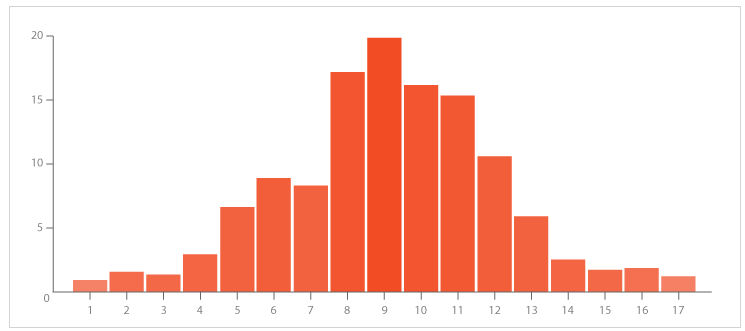
\includegraphics[width=0.4\textwidth]{figures/analysis/histogram.png}%
    \label{fig:analysis:histograms}
    \caption{A histogram is a bar chart over a continuous interval}%
\end{figure}

Histograms visualize the distribution of data over a continuous interval or a certain time period.
A special type is the population pyramid, which is a pair of back-to-back histograms, one for each sex.

Histograms and bar charts expect the same kind of data, i.e.\ a \emph{tabular} data structure.
Almost the same interactions as in Table~\ref{tab:analysis:bar-charts:interactions} can be applied to histograms.
Except a re-ordering of bars along the x-axis.
This is not possible, because the histogram constrains the position of bars along the interval.

\subsection{Bubble charts and scatter plots}

\begin{figure}
  \centering
    \subfloat[Bubble chart]{{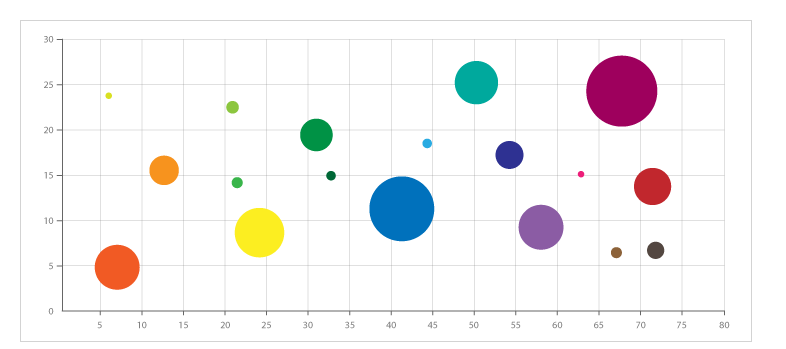
\includegraphics[width=0.4\textwidth]{figures/analysis/bubble-chart.png} }}%
    \qquad
    \subfloat[Scatter plot]{{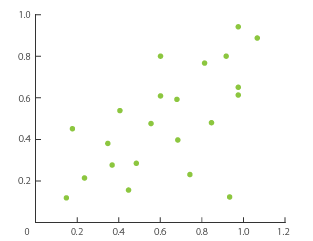
\includegraphics[width=0.4\textwidth]{figures/analysis/scatter-plot.png} }}%
    \caption{Bubble charts and scatter plots are similar regarding interactions}%
    \label{fig:analysis:bubble-chart}
\end{figure}

Both bubble charts and scatter plots are techniques to visualize continuous values from two data attributes.
Points are placed with the two attributes in Cartesian coordinates in order to detect relationships and correlations.

In case of bubble charts, each point is displayed as a bubble with a third value encoded in the size the bubble.
It is even possible to encode a fourth value in the colour of the bubble.

Like line graphs, bar charts and histograms, a scatter plot expects \emph{tabular} data.
Each data point can take up to four values (in case of a coloured bubble chart).
As we can see in Table~\ref{tab:analysis:bubble-charts:interactions}, interactions also include a zooming and movement of the viewpoint.
\begin{table}[H]
  \begin{tabular*}{\textwidth}{lll}
    \bf Category & \bf Description & \bf Exchanged information \\
    \hline
    Select & Highlight a bubble & id of data point \\
    Explore & Zoom in, zoom out & width and height of window \\
    Explore & Move viewpoint position & x- and y-coordinates of viewport \\
    Encode & Change mapping of colour to category & id of data series + colour \\
    Encode & Change colour function & mapping function of value to colour \\
    Encode & Change data attribute to size & mapping function of value to size \\
    Reconfigure & Sort by attribute & data attribute \\
    Reconfigure & Drag bars to reorder data series & ordered list of ids of data series \\
    Filter & Hide a data series & id of data series \\
  \end{tabular*}
  \caption{Plausible interactions for bubble charts}%
  \label{tab:analysis:bubble-charts:interactions}
\end{table}

\subsection{Stacked bar charts}

\begin{figure}
  \centering
    \subfloat[Stacked bar chart]{{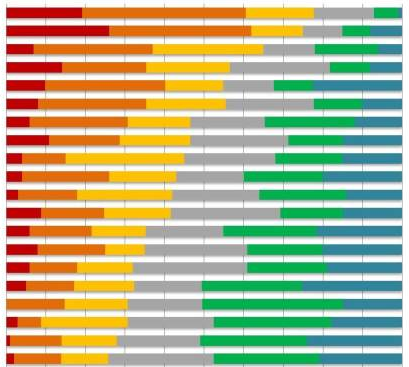
\includegraphics[width=0.3\textwidth]{figures/analysis/stacked-bar-without-baseline.png} }}%
    \qquad
    \subfloat[Stacked bar chart with baseline]{{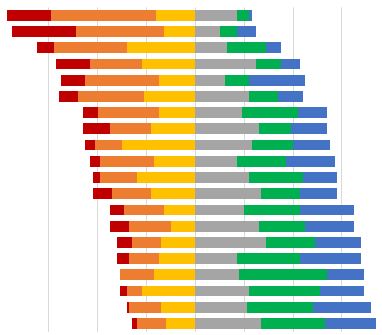
\includegraphics[width=0.3\textwidth]{figures/analysis/stacked-bar-with-baseline.png} }}%
    \caption{Stacked bar charts can be ordered along a baseline or stretch to 100\% width to show the percentage-of-the-whole of each group}%
    \label{fig:analysis:stacked-bar-chart}
\end{figure}
\begin{figure}
  \centering
    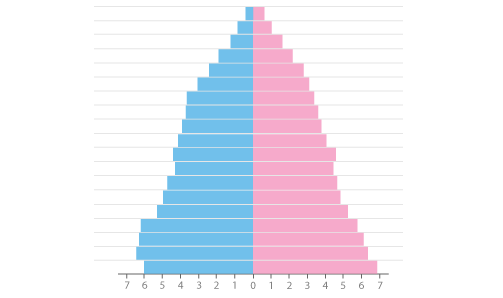
\includegraphics[width=0.4\textwidth]{figures/analysis/population-pyramid.png}%
    \label{fig:analysis:population-pyramid}
    \caption{A population pyramid can be modeled as a stacked bar chart}%
\end{figure}

Unlike a multi-set bar graph which displays bars side-by-side, stacked bar graphs segment their bars of multiple datasets on top of each other.
A baseline, as shown in figure~\ref{fig:analysis:stacked-bar-chart} might be modeled as two back-to-back multi-set bar graphs. A reordering would e.g.\ move one data set from the left side to the right side.

A stacked bar chart also expects \emph{tabular} data.

If the stacked bar chart has a baseline, often the sign of the numeric value defines the placement of the segment on the left or on the right side.
Table~\ref{tab:analysis:stacked-bar-chart:interactions} shows possible interactions, including the highlighting of a data point, a change of color mapping or a reordering of the baseline.
% \conceptTable{Tabular data, multiple date sets as series}{Size, shape, orientation.}{Color, position, texture.}

\begin{table}[H]
  \begin{tabular*}{\textwidth}{lll}
    \bf Category & \bf Description & \bf Exchanged information \\
    \hline
    \bf Select & Highlight a bar & id of data point \\
    \bf Encode & Change mapping of category to colour & id of data series + colour \\
    \bf Reconfigure & Sort by attribute & name of data attribute \\
    \bf Reconfigure & Reorder Y axis & ordered list of ids of data points \\
    \bf Reconfigure & Sort stacking order by attribute & data attribute \\
    \bf Reconfigure & Specify the stacking order data series & ordered list of ids of data series \\
    \bf Reconfigure & Specify a negative data series & list of ids of data series \\
    \bf Filter & Hide a data series & id of data series \\
  \end{tabular*}
  \caption{Plausible interactions for stacked bar charts}%
  \label{tab:analysis:stacked-bar-chart:interactions}
\end{table}


\subsection{Hierarchical visualizations}

\begin{figure}
  \centering
    \subfloat[Tree map]{{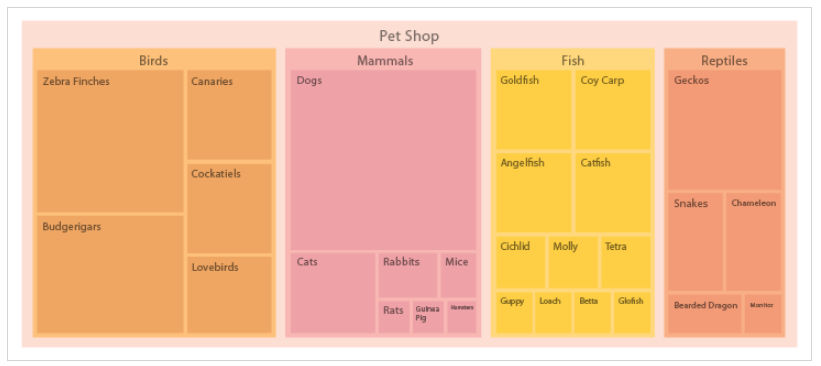
\includegraphics[width=0.4\textwidth]{figures/analysis/treemap.png} }}%
    \qquad
    \subfloat[Sunburst diagram]{{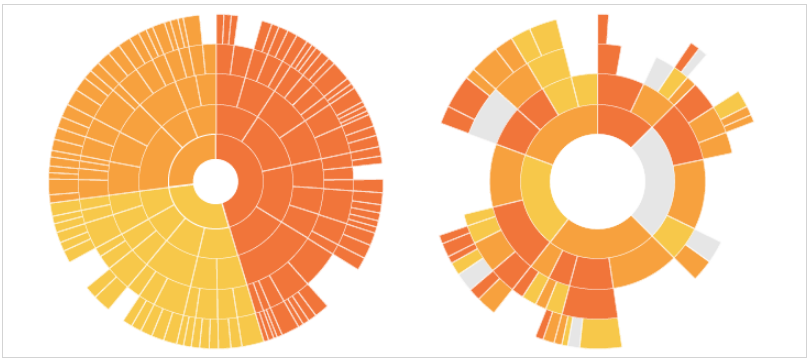
\includegraphics[width=0.4\textwidth]{figures/analysis/sunburst.png} }}%
    \caption{Tree maps and sunburst diagrams are ideal to show hierarchies}%
    \label{fig:analysis:hierarchies}
\end{figure}

Tree maps are great to show hierarchical data without ever exceeding the available screen.
Each feature is a assigned a tile according to a tiling-algorithm.
Unlike a tree map a hierarchical ring diagram or sunburst diagram shows each level of the underlying tree as a series of rings.

Therefore, both tree map and ring diagram expect \emph{hierarchic} data.
Typically, each node will have at least one continuous value that can be used as input for the tiling algorithm or layout algorithm respectively.
Additionally, each node can encode additional attributes by colour.

As these visualization techniques are about hierarchies, the visible, maximal depth of the tree may be increased or decreased.
Again, interactions could include a highlighting of features and a change of color encoding.
Both visualizations may show only a subtree.
E.g.\ a click on a box in the tree map opens another tree map focused on the subtree.
Similarly, a click on a slice of the ring would surround the most external ring with the child nodes of the parent node.
Table~\ref{tab:analysis:hierarchies:interactions} gives a more comprehensive list of interactions.

% \conceptTable{Tree, each feature has a value for layouting.}{Position, Size, shape, orientation.}{Color, texture.}

\begin{table}[H]
  \begin{tabular*}{\textwidth}{lll}
    \bf Category & \bf Description & \bf Exchanged information \\
    \hline
    Select & Highlight a feature & id of data point \\
    Explore & Use another node as root of the visible tree & id of data point \\
    Encode & Change mapping of category to colour & id of data series + colour \\
    Reconfigure & Change data attribute used for layout & name of data attribute \\
    Reconfigure & Sort by attribute & name of data attribute \\
    Reconfigure & Specify order & ordered list of ids of data points \\
    Abstract/Elaborate & Specify maximum depth of visible tree & number of hierarchy levels \\
  \end{tabular*}
  \caption{Plausible interactions for hierarchical visualizations}%
  \label{tab:analysis:hierarchies:interactions}
\end{table}

\subsection{Geographic Data Visualizations}

\begin{figure}
  \centering
    \subfloat[Choropleth map]{{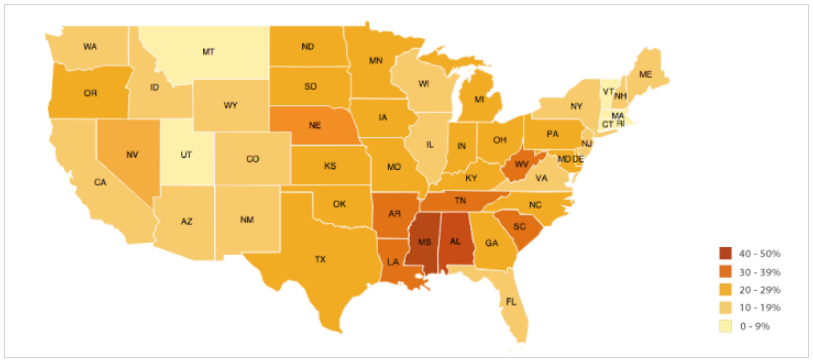
\includegraphics[width=0.4\textwidth]{figures/analysis/choropleth-map.png} }}%
    \qquad
    \subfloat[Flow map]{{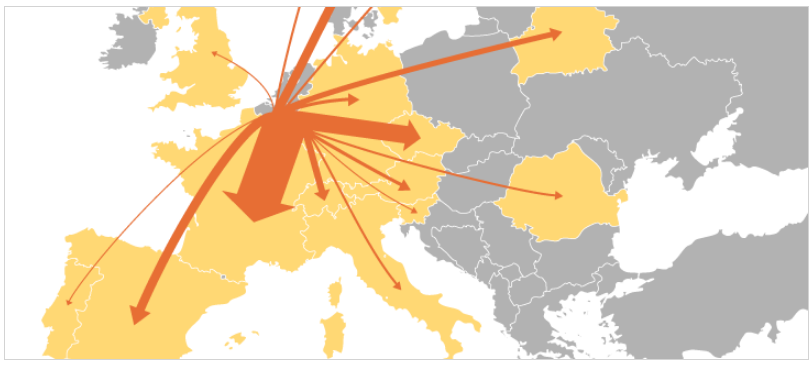
\includegraphics[width=0.4\textwidth]{figures/analysis/flow-map.png} }}%
    \caption{Choropleth maps focus on a density while flow maps show a migration of data}%
    \label{fig:analysis:geographical}
\end{figure}

Choropleth maps and flow maps are thematic maps to visualize geographic data.
Size, position and shape of a data point is determined by its geometry.
Choropleth maps encode a continuous data attribute with relative values in the color of each region.
Flow maps may display relationships between features, a data value defining the size, colour, direction or shape of each arrow.

Non-geographic data may be given in a \emph{tabular} form, assigned to each geographical feature.
In contrast to tabular data, a flow map expects relationships between geographic features.
Thus, it also expects \emph{relational} data in form of a graph

% \conceptTable{Graph data with edges, each feature has geometry data.}{Position, Size, shape, orientation.}{Color, texture.}

\begin{table}[H]
  \begin{tabular*}{\textwidth}{lll}
    \bf Category & \bf Description & \bf Exchanged information \\
    \hline
    Select & Highlight a feature & id of data point \\
    Explore & Move viewport & latitude and longitude of view point \\
    Explore & Zoom in, zoom out & zoom factor \\
    Encode & Change shape of marker & data id  shape \\
    Encode & Change mapping of category to colour & id of data series + colour \\
    Encode & Change colour function & value + colour \\
    Encode & Change data attribute used for colour & name of data attribute \\
    Connect & Show relations of a feature & id of data point  \\
    Abstract/Elaborate & Change granularity of displayed regions & number of hierarchy levels \\
  \end{tabular*}
  \caption{Plausible interactions for geographical visualizations}%
  \label{tab:analysis:geographical:interactions}
\end{table}

\textbf{Activity diagrams}
\begin{figure}
  \centering
    \subfloat[Calendar]{{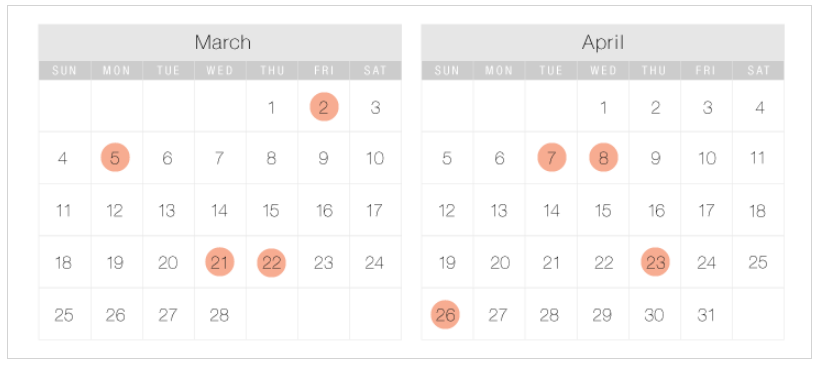
\includegraphics[width=0.4\textwidth]{figures/analysis/calendar.png} }}%
    \qquad
    \subfloat[Gantt chart]{{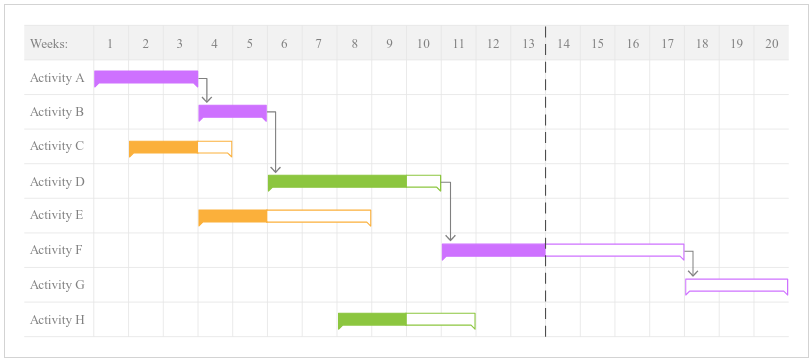
\includegraphics[width=0.4\textwidth]{figures/analysis/gantt-chart.png} }}%
    \caption{Similar to a calendar, a gantt chart shows activities and the progress along a time line}%
    \label{fig:analysis:temporal}
\end{figure}

In activity diagrams, each feature is represented as a rectangle, with the duration of the activity mapped to size and position.
Calendars and gantt charts could not only read the data from the data source, but also add new features to the data set or update metadata of a feature, e.g.\ the progress of the activity.
Calendars and gantt charts expect \emph{tabular} data, although data points might reoccur on a regular schedule.
So some data points, i.e.\ events, might repeat infinitely.

% \conceptTable{Temporal data, each feature has a time interval.}{Position, Size, orientation.}{Color, shape, texture.}

\begin{table}
  \begin{tabular*}{\textwidth}{lll}
    \bf Category & \bf Description & \bf Exchanged information \\
    \hline
    Select & Highlight a feature & id of data point \\
    Explore & Show a different period of dates & start and end datetime \\
    Explore & Show a different time interval & start and end hour\\
    Encode & Change color of categories or activities & id of data series + colour \\
    Encode & Change data attribute used for colour & data attribute \\
    Filter & Remove a calendar or a category & id of data series \\
  \end{tabular*}
  \caption{Interactions for temporal visualizations}%
  \label{fig:analysis:temporal:interactions}
\end{table}

\section{Multiple View Interactions}\label{sec:analysis:examples:multiple}

This section covers examples of multiple data visualizations.
Combination of views are often very specific to certain use cases.
That's why the examples in this section are tied to a use case in contrast to the more generic examples in Section~\ref{sec:analysis:examples:single}.


\textbf{Detail view and Mini View}
\begin{figure}
  \centering
    \subfloat[Detail view]{ 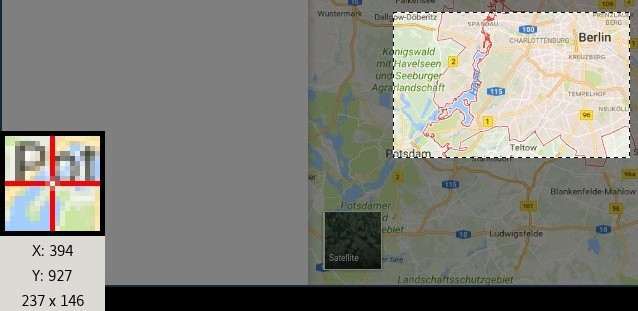
\includegraphics[width=0.4\textwidth]{figures/analysis/detail-view} }%
    \qquad
    \subfloat[Mini view]{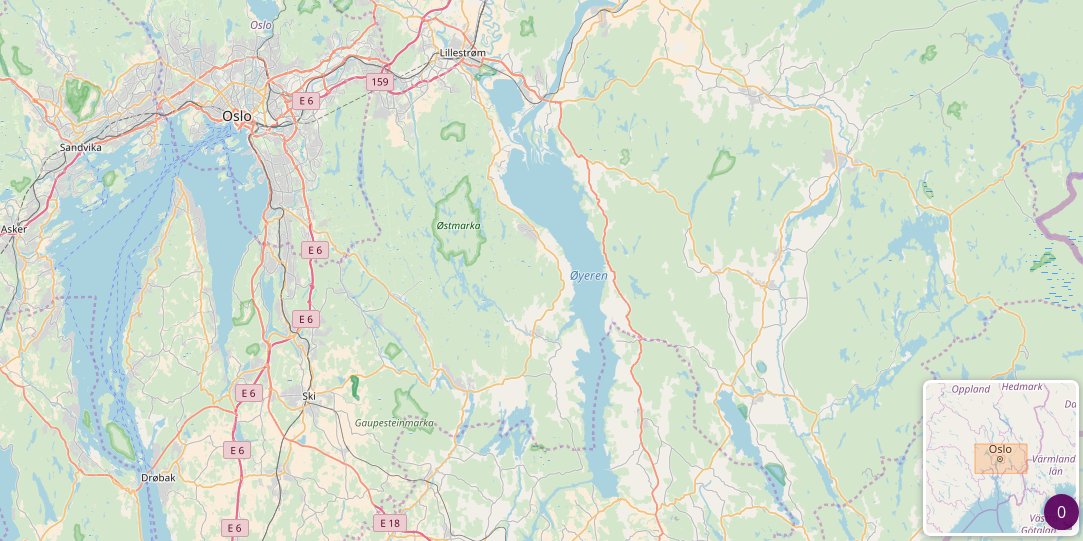
\includegraphics[width=0.4\textwidth]{figures/analysis/mini-view}}%
  \caption{
    The screenshot-tool ``shutter'' shows a magnified detail view of the area around the mouse cursor in the lower left corner of the screen.
  Leaflet-Minimap shows the map at a larger scale in the lower right.
  }
  \label{fig:analysis:detail}
\end{figure}

Detail views show a magnification of the surrounding area of a cursor in a secondary view.
The resolution of the primary view is too high for the user to distinguish individual pixels.
The detail view helps to select items.
Popular use cases are screenshot tools, as seen on the left in Figure~\ref{fig:analysis:detail}, or image processing application.

The opposite of a detail view is the mini view.
You can see an example on the right side of Figure~\ref{fig:analysis:detail}.
This secondary view shows a larger surrounding of the primary view, if the primary view shows only a section of the entire space.
Use cases are geographical visualizations and therefore the expected data structure is a map with coordinates of the viewpoint and a zoom factor for each view.

\begin{table}[H]
  \begin{tabular*}{\textwidth}{lll}
    \bf Category & \bf Description & \bf Exchanged information \\
    \hline
    Explore & Move secondary viewpoint & Latitude + Longitude \\
    Explore & Move primary viewpoint through secondary view & Latitude + Longitude \\
    Explore & Accelerate scrolling via secondary view & Zoom factor \\
  \end{tabular*}
  \caption{Plausible interactions for detail and mini views}%
  \label{fig:analysis:detail:interactions}
\end{table}

\textbf{Timeline}
\begin{figure}
  \centering
    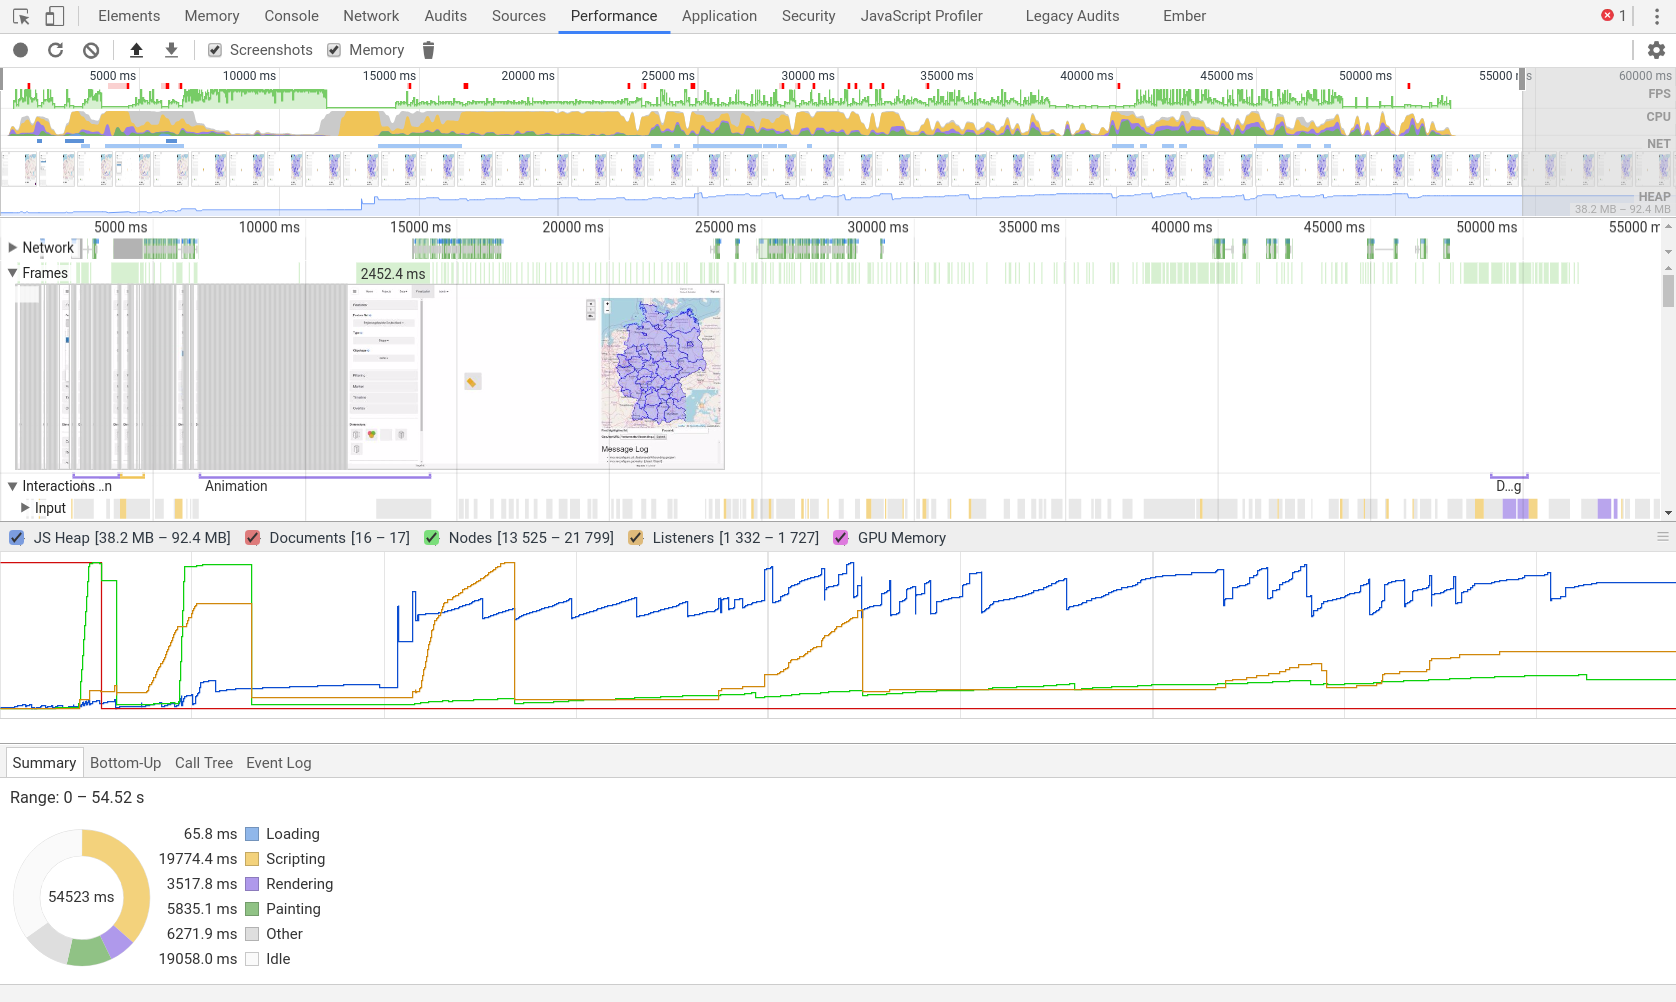
\includegraphics[width=\textwidth]{figures/analysis/profiler}
  \caption{ Multiple views of Chromium's runtime analysis tool can be reduced on a selected time span. }
  \label{fig:analysis:timeline}
\end{figure}
Figure~\ref{fig:analysis:timeline} shows the runtime analysis of the Chromium browser.
Multiple views show different granularities of the same data.
At the top, the entire profiling time frame is visualized, with a screenshot of one step in the middle.
The development of memory is displayed on the third row while a summary is at the very bottom.
The user can select a window on the top line and the data for the other views is reduced on that interval.
A multiple visualization like that expects \emph{temporal} data.

\begin{table}[H]
  \begin{tabular*}{\textwidth}{lll}
    \bf Category & \bf Description & \bf Exchanged information \\
    \hline
    Filter & Filter data by time span & Upper and lower limit \\
    Select & Display screenshot a certain time & Timestamp  \\
  \end{tabular*}
  \caption{Plausible interactions for timelines}%
  \label{fig:analysis:timeline:interactions}
\end{table}





\section{Requirements}\label{sec:analysis:requirements}
In this subsection, a list of formal requirements is imposed on a conceptual \cmv{} framework.
These requirements can be checked in Section~\ref{sec:evaluation} for further evaluation.

\textbf{Serialization} is the process of translating objects that can be stored or transmitted and reconstructed later.
In order to coordinate interactions among views, information needs to be passed from one view to another.
A framework for \cmvs{} should therefore find a serialization format for interactions which has
\begin{enumerate*}[label=(\arabic*)]
  \item
    small payloads and
  \item 
    fast serialization and deserialization.
\end{enumerate*}

\textbf{Reversibility} in the context of a \cmv{} framework means if it is possible to undo the effect of an interaction.
Ideally, every interaction function should have a well-defined inverse.
For every interaction that is not reversible, the computational cost to replay the interactions from the original state up to the point of the interaction should be minimal.

\textbf{Data extensibility} indicates the ease of reloading and updating data on the fly.
This is especially important if an interaction requests additional data from an external service.
We consider good extensibility when
\begin{enumerate*}[label=(\arabic*)]
  \item
    additional data attributes can be added without lookup of corresponding items and
  \item
    no de-duplication steps are necessary when new items are added.
\end{enumerate*}

\textbf{Development costs} qualify how much time and effort is needed in order to develop new components for the \cmv{} framework.
We track these costs in working days and the number of changed lines of code.


\textbf{Maintainability} means in our case, how much other views are impacted by a change of an interaction in one view and how error-prone the framework is.
In general it is hard to measure maintainability.
For the \cmv{} framework we want to measure the
\begin{enumerate*}[label=(\arabic*)]
  \item
    lines of code and the
  \item
    cycliomatic complexity. We will try to find a means to measure
  \item
    cohesion and
  \item
    coupling in the framework.
\end{enumerate*}
The assumption is that the amount of shared data between views is an indicator for high coupling.


\section{Existing Interactions}
In this section, the existing interactions are classified according to the classification by \textcite{Yi2007} of Section~\ref{sec:related-work:interaction-theory:categories}.

In our \visan{} possible interactions can be categorized into the classes \emph{select}, \emph{explore}, \emph{reconfigure}, \emph{encode} and \emph{filter}.

As seen in Figure~\ref{fig:analysis:interaction:existing} the user can \emph{select} one item in the view by clicking on it.
The user can reveal a tooltip showing the item properties by hovering with the mouse on the item, which is another \emph{select} interaction.

The user can \emph{explore} the map in the usual manner:
If the user drags with the mouse on the map, a panning operation is performed with the viewpoint focused on Germany, i.e.\ the camera moves around like a turntable.
The zoom factor can be changed by scrolling on the canvas of the map.

\emph{Encode} and \emph{reconfigure} techniques are performed through the menu on the left side:
Under the ``features'' tab, the user can \emph{reconfigure} different data sets and the displayed diagram, e.g.\ a tree map visualization based on the geometry shape, cubes or voronoi regions.
The tab ``Dimensions'' allows the user to \emph{encode} properties of a data set to visual attributes, e.g.\ the height, color and texture of an item.

The tab ``Filter'' can be used to reduce the displayed data set along a range of continuous values.
Figure~\ref{fig:analysis:interaction:existing:filter} shows the range of visible values in the left menu.
When the user drags the slider, the items in the map on the right side are \emph{filtered} accordingly.

\begin{figure}[h]
  \centering
  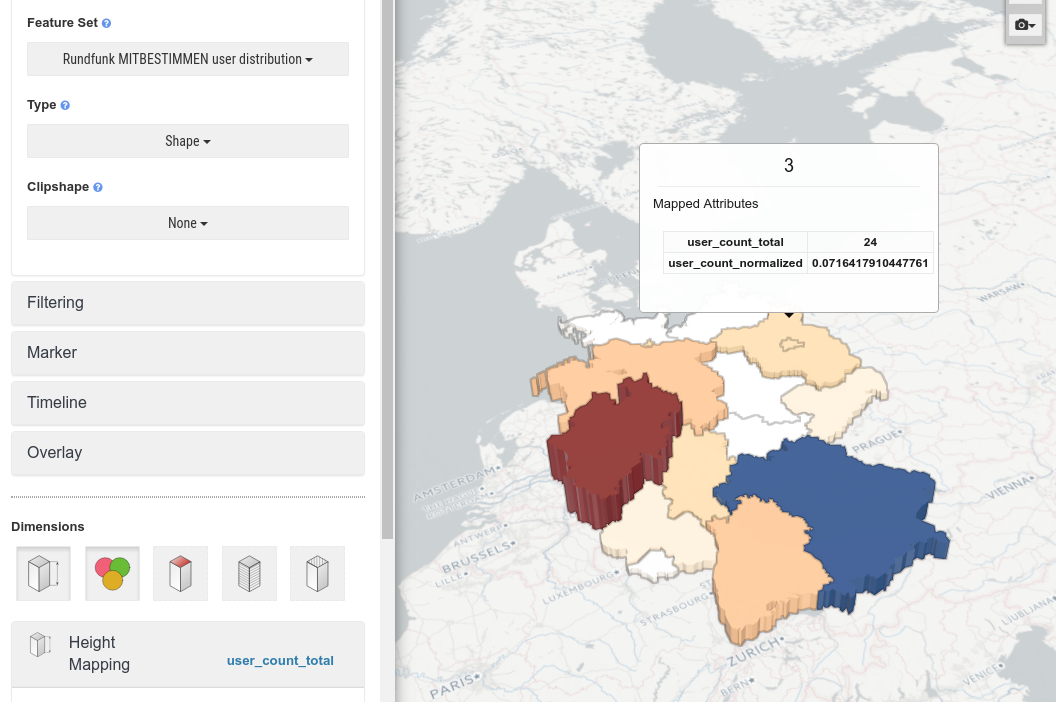
\includegraphics[width=\textwidth]{images/existing-interactions.png}
  \caption{%
    Items can be highlighted with a click, Bavaria is currently highlighted.
    A mouse over reveals a tooltip showing item properties.
    The menu on the left side allows to change the data set and the specific base visualization.
  }\label{fig:analysis:interaction:existing}
\end{figure}

\begin{figure}[h]
  \centering
  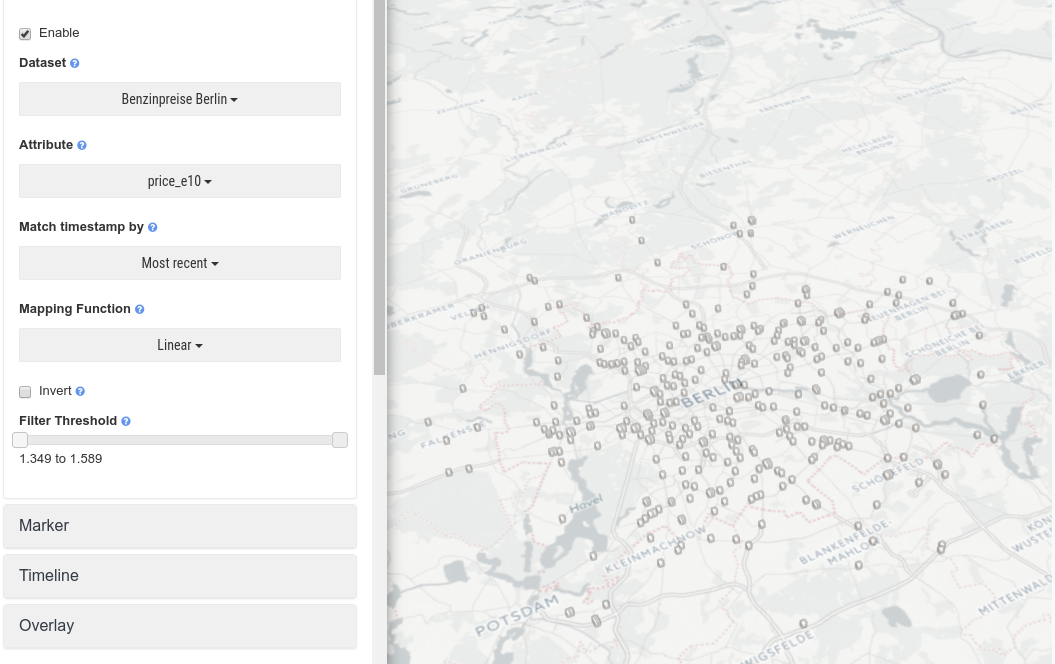
\includegraphics[width=\textwidth]{images/existing-interactions-filter.png}
  \caption{%
    Only gas stations with a price for E10 within 1.349 Euro and 1.589 Euro are displayed in the map
  }\label{fig:analysis:interaction:existing:filter}
\end{figure}

\section{Comparison of client-side component frameworks}\label{sec:analysis:frontend-framework-comparison}

This section evaluates the most suitable client-side rendering and component based JavaScript framework for \cmvs{} and whether or not to use web components.

Three JavaScript frameworks have been evaluated:
\begin{enumerate*}[label=(\arabic*)]
  \item GlimmerJS
  \item Google Polymer and
  \item ReactJS.
\end{enumerate*}
Google Polymer is built on top of web components and GlimmerJS applications can be exported as a web component, but React does not support web components.

Critically, \cmvs{} require a means to exchange data between views, which is specific to interactions.
The web component specification, unfortunately, does not specify how arbitrary JavaScript objects can be passed to web components.
String based attributes are supported, as seen in Listing~\ref{lst:evaluation:web-components-data}.

To pass rich data to components however, web component frameworks have to roll their own data flow and syntax.
Google Polymer's syntax to pass rich data to a components is shown in Listing~\ref{lst:evaluation:polymer-data}.
But this is a proprietary solution that abandons standard HTML.


\lstinputlisting[
  language=HTML,
  label={lst:evaluation:web-components-data},
  caption={An example of string based attributes of web components~\cite{GoogleMapWebComponent2017}}
]{listings/evaluation/web-components-data.html}

\lstinputlisting[
  language=HTML,
  label={lst:evaluation:polymer-data},
  caption={An small syntax example how Google Polymer passes rich data to a component}
]{listings/evaluation/polymer-data.html}

This raises some problems in existing applications:
A particular component-based frontend framework can not be assumed, a lot of existing applications are also written without any JavaScript framework.
Proprietary solutions like the one of Polymer reduce the main motivation of implementing against web components:
Platform agnostic flexibility.

As a summary, if there is
\begin{enumerate*}[label=(\arabic*)]
  \item no obligation to implement web components
  \item and an easy integration into an existing application is necessary,
\end{enumerate*}
then React is the perfect choice for \cmvs{}.

Figure~\ref{fig:implementation:frontend-frameworks} shows the pros and cons of each framework for the use case.

\begin{figure}[h]
  \centering
  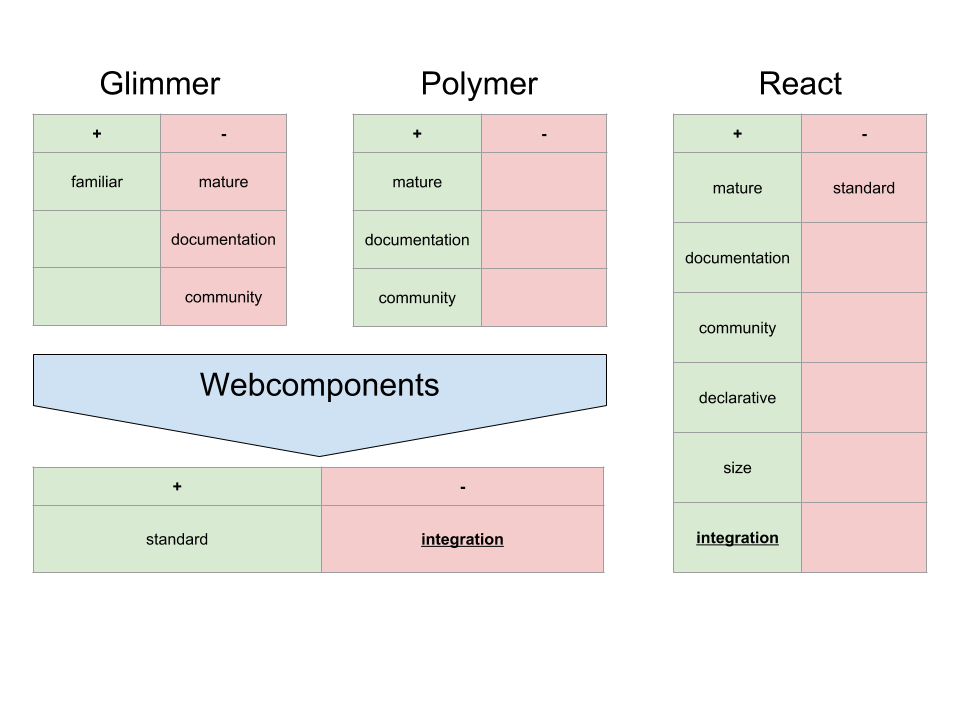
\includegraphics[width=\textwidth]{images/frontend-frameworks.png}
  \caption{Comparison of component based web frameworks, advantages highlighted in green, disadvantages highlighted in red.}\label{fig:implementation:frontend-frameworks}
\end{figure}

